\chapter{Informacje ogólne}
\label{cha:Lab001}
\makeatletter


% *********************************************************************
% w poniższej metryczce należy uzupełnić informacje o:
% - temacie ćwiczenia
% - numer ćwiczenia
% - numer grupy laboratoryjnej
% - numer zespołu
% - datę wykonania ćwiczenia oraz oddania ćwiczenia.
% *********************************************************************

\begin{table}[H]
    \centering
    \renewcommand{\tabularxcolumn}[1]{m{#1}}  % Dostosowanie kolumny do zawartości
    \newcolumntype{C}{>{\centering\arraybackslash}X}
    \begin{tabularx}{\linewidth}{|C|C|}
        \hline
        \multicolumn{2}{|c|}{\makecell{\textbf{\Large{Biometryczne Systemy Zabezpieczeń}} \\ \textbf{Projekt}}} \\ \hline
        \multicolumn{1}{|l|}{Temat}                    &           Weryfikacja głosowa na stronie internetowej                \\ \hline
        \multicolumn{1}{|l|}{Technologie}                       &       Python, JavaScript, framework - Flask, narzędzie FFmpeg               \\ \hline
        \multicolumn{1}{|l|}{Biometryka}                    &           Voice             \\ \hline
        \multicolumn{1}{|l|}{Autorzy}                         &   \@author                              \\ \hline
        \multicolumn{1}{|l|}{Grupa laboratoryjna}                       &       02               \\ \hline
        
        
    \end{tabularx}
\end{table}


\section{Opis ogólny projektu}
Celem projektu jest przedstawienie komponentu biometrycznego - voice. Głos człowieka może być zastosowany jako unikalne zabezpieczenie (np. podczas logowania, lub innego zabezpieczenia zasobów). Komponent ten został zaimplementowany na stronie internetowej jako zabezpieczenie konta użytkownika. Użytkownik ma możliwość nagrać próbkę swojego głosu z wypowiadając daną frazę, a następnie przechodząc do logowania nagrywa ponownie próbkę głosu z tą samą frazą, po czym następuje weryfikacja. Obsługa komponentu biometrycznego została napisana w pythonie z użyciem odpowiednich bibliotek, a prosta witryna internetowa do jego wykorzystania została napisana we frameworku pythona - Flask. 

\section{Wstęp teoretyczny}

Głos jest jednym z wyjątkowych i bardzo ciekawym narzędziem, które może mieć bardzo szerki zakres zastosowań w zabezpieczeniach biometrycznych. Łączy on w sobie dwa aspekty, które wpływają na jego unikalność:

\begin{itemize}
	\item Cechy fizyczne głosu - w tym punkacie zawarte są na przykład kształt i rozmiar traktu głosowego, strun głosowch i płuc. Podobnie jak inne części ciała wykorzystywane w biometrii (np. tęczówka, linie papilarne), te cechy głosu są również dla każdego człowieka unikalne.
	\item Cechy behawioralne - na te cechy wpływa akcent, tonacja, rytm czy tempo. Są to cechy które wykształciły się na przeztrzeni lat u każdej osoby.
\end{itemize}
W projekcie wykorzystywana jest kombinacja obu tych aspektów, aby stworzyć koncepcję systemu, który mógłby zostać częściej wykorzystywany jako główne zabezpieczenie zasobów.
\newline
\newline
Projekt ten działa w dwóch fazach:

\subsection{Rejestracja}
W tej fazie system najpierw potrzebuje wzorca bimetrycznego, który będzie później wykorzystywany w głównej fazie projektu.
\\
\\
\textbf{Pobranie danych}\newline
Użytkownik wypowiada swoje hasło (frazę potrzebną później do weryfikacji). Mikrofon w komputerze przetwarza fale ciśnienia akustcznego na sygnał elektryczny. Natępnie przeglądarka przy pomocy skryptu (JavaScript) digitalizuje go i koduje na format \textbf{.webm}
\newline
\\
\textbf{Pzetwarzanie wstępne}\newline
W tym kroku surowy plik .webm jest przesyłąny do analizy. Wykorzystywana jest biblioteka \textbf{pydub}, aby przekształcić ten plik do formatu .wav z częstotliwością 16000Hz i kanałem mono. Jest to działanie istotne by zachować spójność.
\newline
\\
\textbf{Wydobycie cech biometrycznych}\newline
Jest to najważniejszy krok w projekcie. System nie porównuje bezpośrednio plików dźwiękowych, ponieważ byłoby to nieefektywne. Z tego powodu z sygnału audio wydobywane są jego cechy charakterystyczne. W przypadku tego projektu są to \textbf{Współczynniki Cepstralne w Skali Mel (MFCC)}.
\newline
\\
\textbf{Współczynniki Cepstralne w Skali Mel (MFCC)} - jest to zbiór kilkunastu liczb które w połączeniu tworzą numeryczną reprezentację barwy dźwięku w krótkim fragmencie czasu.
\newline
\\
W programie najpierw następuje wczytanie pliku .wav jako talibcy liczb (numpy). Następnie z sygnału usuwana jest cisza, by system skupił się tylko na głównej części czyli wypowiedzianej frazie. Na końcu biblioteka Librosa analizuje sygnał klatka po klatce, w bardzo krótkich fragmentach i dla każdej z nich oblicza 13 współczynników MFCC. Liczby te opisują kształt widma, czyli barwę dźwięku w sposób, który jest odporny na zmiany głośności i tonu.
\newline
Efektem tych działań jest wydobyty wzorzec biometryczny - macierz cech. Jest to tabela liczb, w której wiersze to kolejne ramy czasowe a kolumny to współczynniki MFCC.
\newline
\\
\textbf{Zapisanie wzorca}\newline
W tym projekcie dla uproszczenia zapisujemy cały plik .wav. Za każdym razem gdy system potrzebuje wzorca, cechy są z niego wydobywane na nowo

\subsection{Weryfikacja}
W tej fazie następuje weryfikacja, czy nowa próbka głosu jest podobna do zapisanego wzorca.
\\
\\
\textbf{Dla próbki do weryfikacji punkty: pobranie danych, przetwarzanie wstępne i wydobycie cech biometrycznych są powtarzane.}
\\
\\
Teraz system mając dwie macierze cech z obu próbek musi je porównać. Na tym etapie jednak pojawia się pewien problem, gdyż użytkownik, mimo że będzie to ta sama osoba, nigdy nie powtórzy idealnie i w tym samym tempie wypowiedzianej frazy. By rozwiązać ten problem w projkecie został wykorzystany alogorytm \textbf{Dynamicznego Dopasowania Czasu - DTW}.
\\
\\
\textbf{Alogorytm Dynamicznego Dopasowania Czasu - DTW} - jest to metoda służąca porównaniu dwóch sekwencji (w tym przypadku czasowych), która potrafi poradzić sobie z różnicami w tempie.
Głównym zadaniem tego algorytmu jest znalezenie optymalnego dopasowania między elemetnami jednej sekwencji a drugiej, by łączna różnia między dopasowanymi elementami była jak najmniejsza.
\\
\\
W pierwszej kolejności tworzona jest mapa kosztów lokalnych. W tym celu wykorzystywana jest funkacja \textbf{cdist} z biblioteki scipy. Tworzy ona macierz, gdzie każda komórka zawiera informację jak bardzo różni się i-ta ramka z pierwszego nagrania od j-tej ramki z drugiego nagrania. Dzieje się to poprzez obliczanie dystansu euklidesowego między współczynnikami MFCC.
\newline
\\
Następnie algorytm DTW przechodzi przez macierz kosztów i znajduje ścieżkę o najmniejszym łącznym koszcie. Im ta wartość jest mniejsza tym głosy są bardziej podobne.
Efektem jego działania jest skumulowany dystans. Jest to finalny wynik porównania biometrycznego.
\\
\\
Ostatni punkt to określenie na podstawie prostego warunku logicznego czy obliczona odległość jest wyższa lub niższa od skalibrowanego wcześniej progu decyzyjnego na podstawie którego użytkownik jest zweryfikowany lub nie.  

\section{Opis wykorzystywanego oprogramowania i narzędzi}
\begin{itemize}
	\item \textbf{Python} - główny język programowania na którym opiera się cały projekt
	\item \textbf{JavaScript} - język skyrptowy, który posłuzył do stworzenia systemu nagrywania głosu (dynamicznie działające przyciski, zapisywanie głosu w danym formacie)
	\item \textbf{Flask} - framework Pythona który posłużył do stworzenia szaty graficznej projektu (strony internetowej na której odbywa się weryfikacja głosowa)
	\item Biblioteki Pythona
	\begin{itemize}
		\item \textbf{numpy} - jest jedną z głównych elementów projektu. Wykorzystana została do stworzenia tablicy jednowymiarowej w której przechowywane są liczby zmiennoprzecinkowe stworzone przez inną bibliotekę librosa, reprezentujące głos. Potrzebna jest również do uproszczenia operacji matematycznych oraz pozwala na zarządzanie macierzami zawartymi w kodzie
		\item \textbf{librosa} - biblioteka ta w projekcie ma szczególnie zadanie, odpowiada ona za cały aspekt analizy dźwięku. Dzięki niej wczytywany jest głos oraz dekodowany, wstępnie oczyszcza dźwięk (np. usuwa sekundy ciszy z nagrania) oraz najważniejsze odpowiada za wydobycie cech biometrycznych z głosu.
		\item \textbf{SciPy  moduł scipy.spatial.distance} - biblioteka ta to olbrzymi zbiór gotowych maszyn i narzędzi matematycznych, inżynierskich i naukowych
		\item \textbf{pydub} - ta biblioteka posłużyła jako narzędzie do manipulacji i przetwarzania plików audio. W kontekście projektu jej główna rola to przyjmowanie plików głosowych, a następnie konwertuje je do formatu WAV. 
		\item \textbf{os} - biblioteka ta posłużyła do obsługi plików i folderów
		
	\end{itemize}	
\end{itemize}	



\section{Działanie programu}
Najważniejszą rzeczą przed uruchomieniem projektu jest pobranie i dodanie do zmiennych środowiskowych narzędzia FFMPEG. Jest ono potrzebne do poprawnego działania biblioteki pydub.
\newline
Działanie projektu zaczyna od strony głównej na której jest rejestracja i logowanie. W pierwszym kroku użytkownik rejestruje się nagrywając próbkę głosu. 

\begin{figure}[H]
	\centering
	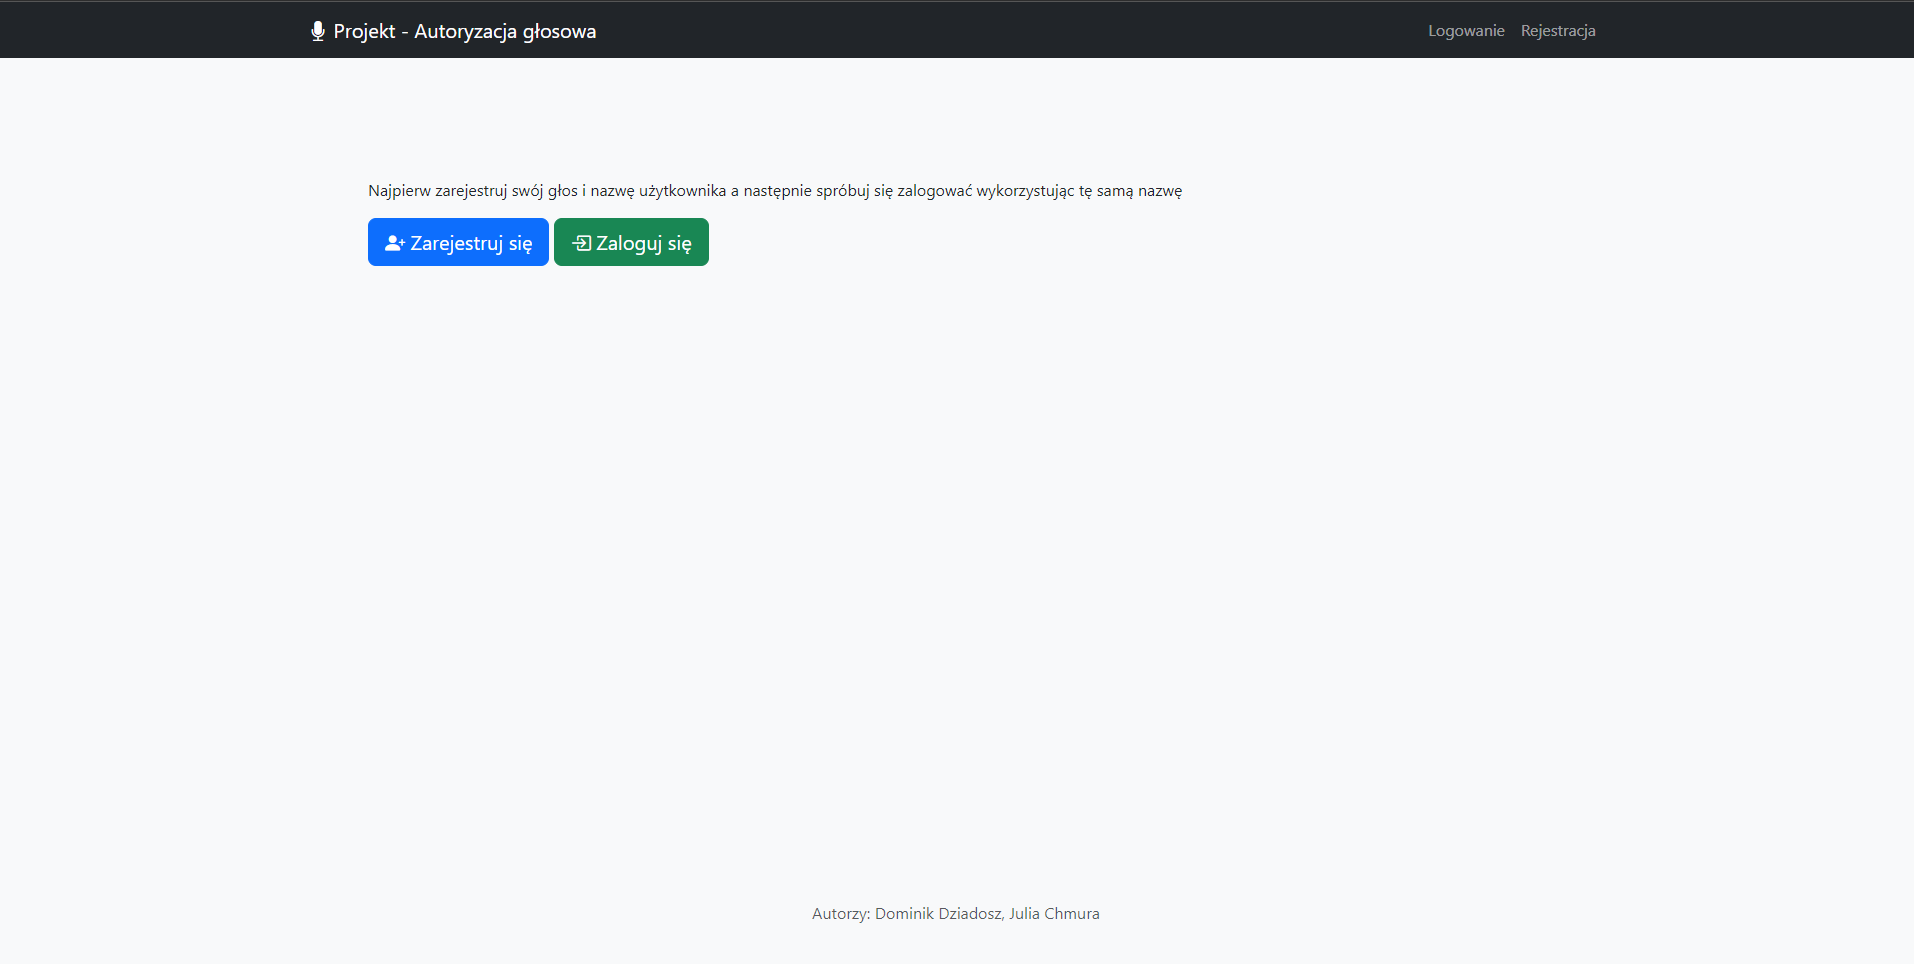
\includegraphics[width=\linewidth]{src/images/strona_glowna.png}
	\caption{Obraz strony głównej}
\end{figure}

Po kliknięciu "Zarejestruj się" przechodzimy do strony rejestracji. Tutaj podawana jest nazwa użytkownika i nagrywana próbka głosu (około 2 do 3 sekundy). 

\begin{figure}[H]
	\centering
	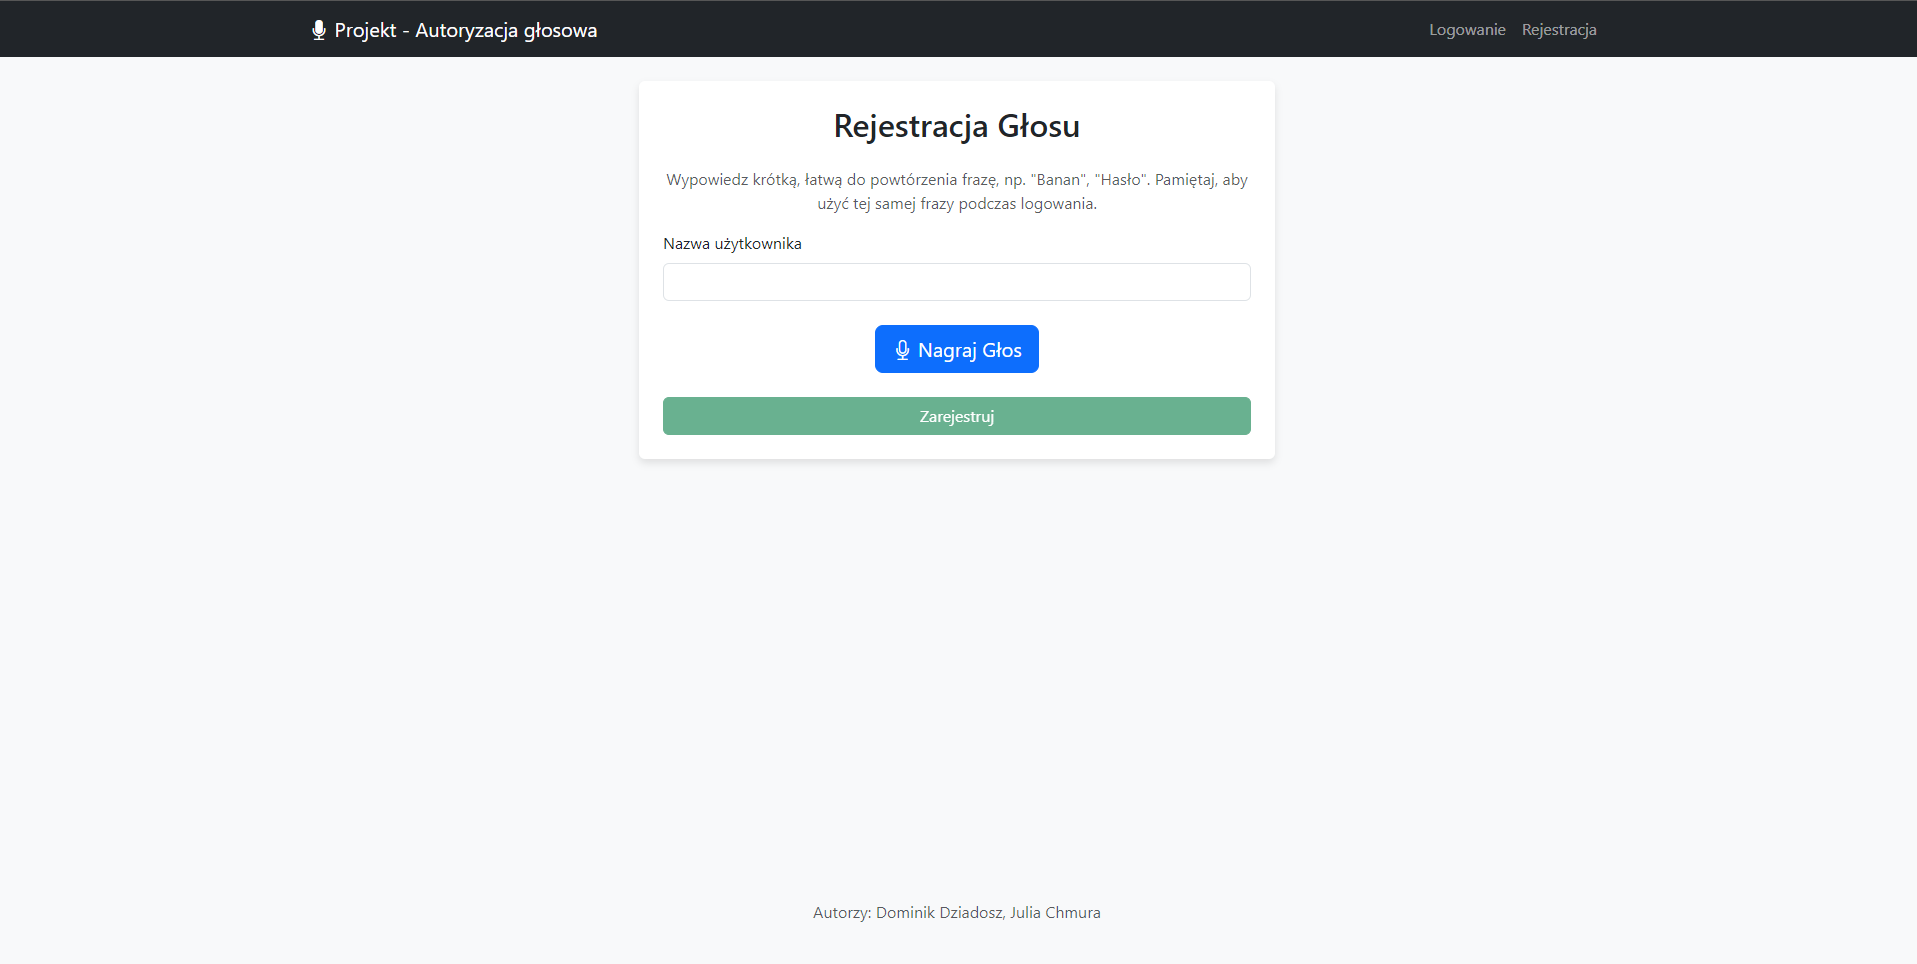
\includegraphics[width=\linewidth]{src/images/nagranie_probki_glosu.png}
	\caption{Obraz strony rejestracji}
\end{figure}

Po zarejestrowaniu się należy przejść do logowania. Tutaj ponownie podajemy nazwę użytkownika i nagrywana jest kolejna próbka, która jest porównywana do tej podanej podczas rejestracji. Jeżeli próbki będą zgodne, użytkownik przechodzi poprawnie przez weryfikację lub nie przechodzi, w każdym przypadku zostaje o tym poinformowany stosownym komunikatem. 

\begin{figure}[H]
	\centering
	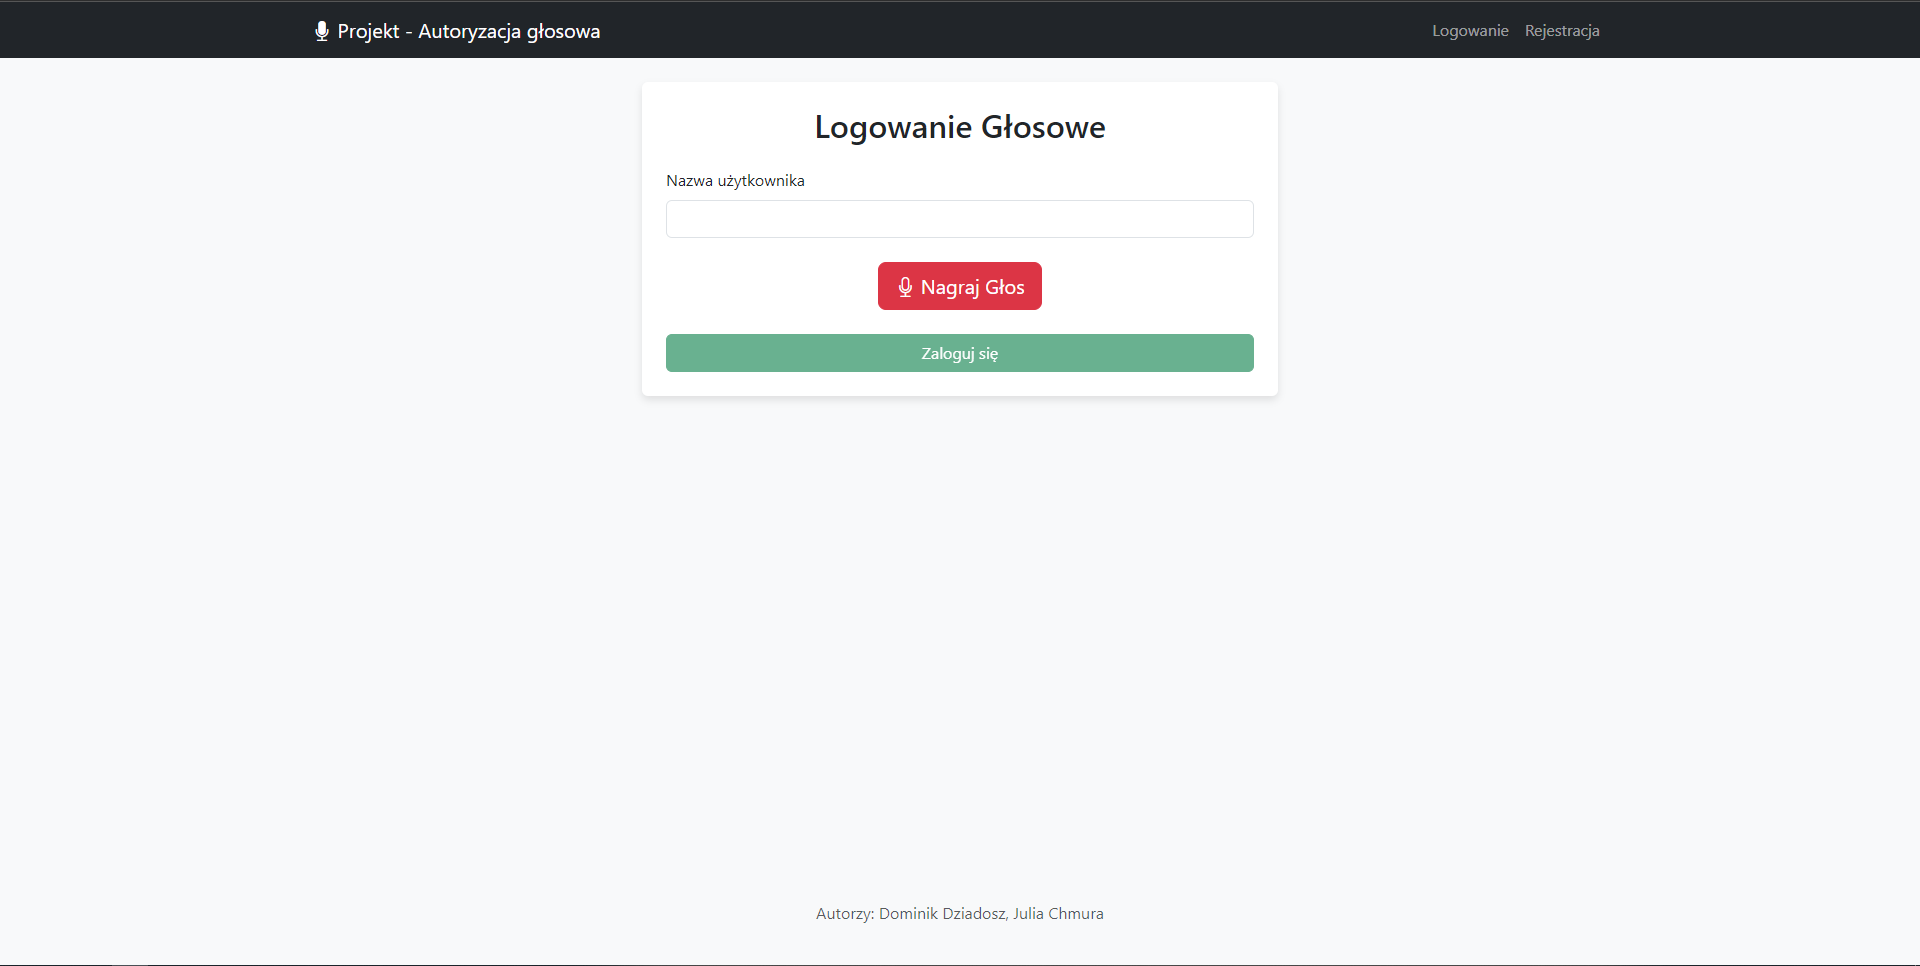
\includegraphics[width=\linewidth]{src/images/weryfikacja_probki_glosu.png}
	\caption{Obraz strony logowania}
\end{figure}

\section{Instrukcja nagrywania próbki głosu}
Aby poprawnie nagrać próbkę głosu należy spełnić dane warunki:
\begin{itemize}
	\item Przygotować odpowiedni sprzęt: poprawnie działający mikrofon
	\item Mówić jednolitym tonem 
	\item Wypowiedzieć proste hasło, najlepiej zkładające się z jednego lub dwóch słów
	\item Przy rejestracji i logowaniu posłużyć się tym samym zwrotem, mówiąc w takim samym tonie i tempie
	\item Upewnić się że nagrania nie zakłucają odgłosy z otoczenia
	\item Nagrać próbkę trwającą około dwie lub trzy sekundy
	
\end{itemize}


\section{Wnioski}
Na podstawie przeprowadzonych eksperymentów można stwierdzić, że:
\begin{itemize}
    \item Histogram jest przydatnym narzędziem w analizie jakości obrazu biometrycznego.
    \item Wyrównanie histogramu poprawia kontrast i może zwiększać czytelność obrazu.
    \item Segmentacja oparta na histogramie, w szczególności metoda Otsu, pozwala na skuteczne wydzielenie istotnych cech obrazu.
\end{itemize}

\section{Bibliografia}
\begin{itemize}
    \item MATLAB Image Processing Toolbox Documentation \cite{mathworks},
    \item Rafael Gonzalez, Richard Woods, Digital Image Processing Global Edition \cite{gonzalez2017}.
    \item Flask Documentation. Pallets.  \cite{flask_docs}
    \item Pydub Documentation. Read the Docs.  \cite{pydub_docs}
    \item Librosa Documentation  \cite{librosa_docs}
    \item SciPy Documentation  \cite{scipy_docs}
    \item NumPy Documentation \cite{numpy_docs}
    \item scikit-learn Documentation  \cite{scikitlearn_docs}
    \item FFmpeg Documentation  \cite{ffmpeg_docs}
    
\end{itemize}
